
\documentclass[a4paper,12pt]{article}
\usepackage[utf8]{inputenc}
\usepackage[english,russian]{babel}
\usepackage[T2A]{fontenc}
\usepackage{mathtext}
\usepackage{gauss}
\usepackage{graphicx}
\usepackage{amsmath, amsfonts, amssymb}
\newtheorem{theorem}{Теорема}
\usepackage[left=2.50cm, right=2.00cm, top=2.00cm, bottom=2.00cm]{geometry} 
\usepackage{mathdots} 
\usepackage[pdftex]{lscape}
\usepackage{mathtools}
\usepackage{pgfplots}
\pgfplotsset{compat=1.9}
\usepackage{graphicx}%Вставка картинок правильная
\usepackage{tikz}
\usepackage{float}%"Плавающие" картинки
 \usepackage{relsize}
\usepackage{wrapfig}%Обтекание фигур (таблиц, картинок и прочего)
\usepackage{ tipa }
\usepackage{amsmath}
  \usepackage[unicode=true, colorlinks=true, linkcolor=blue, urlcolor=blue]{hyperref}
\linespread{1}
\newcommand{\om}{\overline{o}}
\newcommand{\OB}{\underline{O}}
\newcommand{\eps}{\varepsilon}
\newcommand{\RR}{\mathbb{R}}
\newcommand{\NN}{\mathbb{N}}
\newcommand{\CC}{\mathbb{C}}
\newcommand{\QQ}{\mathbb{Q}}
\newcommand{\ZZ}{\mathbb{Z}}
\newcommand{\dx}{\d{dx}}
\newcommand{\ph}{\varphi}
\newcommand{\F}{\mathbb{F}}
\newcommand{\E}{\mathbb{E}}
\begin{document}
	\section*{1}
	$$Q(x_1,x_2, x_3, x_4) = 25x^2_1 + 3x^2_2 - 9x^2_3 -20x_1x_2 -30x_1x_3 + 6x_2x_3$$
	Запишем матрицу соотвествующей биленейную форму и приведем ее к диагональному виду с помощью симметричного Гаусса.
	$$\begin{pmatrix}
		-25 & -10 & -15 \\
		-10 & 3 & 3 & \\
		-15 & 3 & -9
	\end{pmatrix}\overset{\hat{\text{э}}_1(2, 1, +1),\, }{\mathlarger{\mathlarger{\leadsto}}} \begin{pmatrix}
	25 & 15 & -15  &| &1 & 0 & 0\\
	15 & 8 & -12&| &1 & 1 & 0\\
	15 & -12 & -9 &|&0 & 0 & 1
	\end{pmatrix}\overset{\hat{\text{э}}_1(3, 2, +1),\, }{\mathlarger{\mathlarger{\leadsto}}}$$
	$$\begin{pmatrix}
		25 & 15 & 0 & | & 1 & 0 & 0 \\
			15 & 8 & -4 & | & 1 & 1 & 0 \\
				0 & -4 & -2 & | & 1 & 1 & 1 \\
	\end{pmatrix}\overset{\hat{\text{э}}_1(2, 1, -3/5),\, }{\mathlarger{\mathlarger{\leadsto}}}$$
	$$\begin{pmatrix}
		25 & 0& 0 & | & 1 & 0 & 0 \\
				0 & -1 & 0 & | & 2/5 & 1 & 0 \\
						0 & 0 & 9 & | & 1 & 1 & 1 \\
	\end{pmatrix}\rightsquigarrow\begin{pmatrix}
		1 & 0& 0 & | & 1/25 & 0 & 0 \\
0 & -1 & 0 & | & 2/5 & 1 & 0 \\
0 & 0 & 1 & | & 1/9 & 1/9 & 1/9 \\
	\end{pmatrix}$$
	Матрица, записанная справа, это матрица перехода, только траспонированная. 
	$$C = \begin{pmatrix}
		1/25 & 2/5 & 1/9 \\
		0 & 1 & 1/9 \\
		0 & 0& 1/9
	\end{pmatrix}$$
	\section*{2}
	Запишем матрицу билинейной формы\\ $$Q(x) = -3x_1^2+(-b-8)x^2_2+(-9b+8)x^2_3+ 8x_1x_2 + 2x_1x_3 + 2(3b-3)x_2x_3$$
	$$\begin{pmatrix}
		-3 & 4 & 1 \\
		4 & -b-8 & 3b-3 \\
		1 & 3b-3 & -9b-8
	\end{pmatrix}$$
	 Посчитаем все угловые миноры: \\
	 1) $\delta_1 = -3$\\
	 2)  $\delta_2 = 3(-b-8)-16 = 3b+8$\\
	 3)  $\delta_3 = -3(b+8)(9b+8) + 4(3b-3) + 4(3b-3) + (3b-3)^2(-3) + (9b+8)16 = -125b-53$
	 Теперь мы можем выписать нормальный вид, в зависимости от параметра $b$ \\
	 $b = -\frac83$: $-x^2_1-x_3^2$\\
	 $b = -\frac{53}{125} : -x^2_1+x_2^2$ \\
$-\frac83 < b< -\frac{53}{125}: -x^2_1-x_2^2-x^2_3$  
	 $b = -\frac83$: $-x^2_1-x_3^2$\\
$b >-\frac{53}{125}: -x^2_1+x_2^2+x^2_3$ \\
$b <-\frac{8}{3}: -x^2_1-x_2^2-x^2_3$ 
\section*{3}
\subsection*{a)}
$$Q(f) = \int\limits_0^2f^2(x)\d{dx} - \int\limits_{1}^{3}f^2(x)\dx$$
Посчитаем значение функции на векторе $v = a+bx+cx^2+dx^3$
$$Q(v) = \int\limits_0^2v^2\d{dx} - \int\limits_{1}^{3}v^2\dx = -4ab-12ac-32ad-6b^2-32bc-84bd-42c^2-\frac{664}{3}cd -294d^2$$
Получился однородный многочлен степени 2, а значит функция является квадратичной формой.
\section*{4} 
Чтобы билинейная форма задавала скалярное произведение, небходимо, чтобы матрица это формы была симметрична и положительно определена. Запишем матрицу этой билинейной формы.
$$\begin{pmatrix}
	-4b+13 & -2b+6 & -a+2.5\\
	-2b+6 & 2 & -2b+4 \\
	-2b+5 & -2b+4 & 3 
\end{pmatrix}$$
Чтобы матрица была симметрична, необходимо $-a+2.5 = -2b+5 \to a = 2b-2.5$\\
Чтобы матрица была положительно определенной, необходимо, чтобы каждый угловой минор не меньше нуля\\
$$\begin{cases}
$$\delta_1 = -4b+13\geqslant0$$ \\
$$\delta_2 = -4b^2+16b-10\geqslant0$$ \\
\delta_3 = 192b^3-732b^2+336b+82\geqslant0
\end{cases}$$
$\delta_3 = (-4b+13)(2)(3)+ (-2b+6)(-2b+4)(-2b+6)+ (-2b+5)(-2b+6)(-2b+4)- 2(-2b+5)^2-(-2b+4)^2(-4b+13)\-3(-2b+6)^2$
$$\begin{cases}
	$$\delta_1 = -4b+13\geqslant0$$ \\
	$$\delta_2 = -4b^2+16b-10\geqslant0$$ \\
	\delta_3 = 192b^3-732b^2+336b+82\geqslant0
\end{cases}\leftrightarrow \begin{cases*}b\in{\left[\frac{4-\sqrt6}{2},\frac{4+\sqrt6}{2}\right]} =I\\
192b^3-732b^2+336b+82\geqslant0 \end{cases*}\to $$
$$b \in \left[\frac{63+\sqrt{2377}}{48}, \frac{4+\sqrt{6}}{2}\right]$$
Значение $192b^3-732b^2+336b+82$ на концах интревала I равно $-8$. в этом интревале  есть точка перегиба, то есть функция сначала убывала, потом возрастала или наоборот. Точка перегиба в точке $\frac{61}{48}$.Локальные эксремумы в точках $\frac{61-\sqrt{2377}}{48}, \frac{61+\sqrt{2377}}{48}$
\begin{figure}[h]
	
	\centering
	
	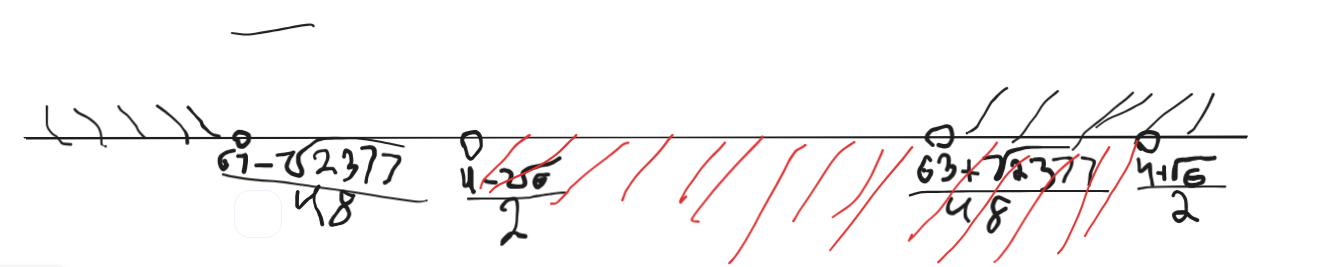
\includegraphics[width=0.8\linewidth]{ИДЗ_?.png}
	
	\caption{Пересечение отрезков}
	
	\label{fig:mpr}
	
\end{figure}
\section*{5)}
Заметим, что каждый минор неотрицателен и матрица симметрична, значит матрица является матрицей Грама какой-нибудь системы векторов. \\
Запишем матрицу и приведем ее к диагональнмоу виду, с помощью симметричного Гаусса, но слева запишем единчнкую матрицу, чтобы сохранить все преобразования.
$$\begin{pmatrix}
	17 & 12 & -87 \\
	12 & 18 & -90 \\
	-87 & -90 & 531
\end{pmatrix}\overset{\hat{\text{э}}_1(2, 1, -\frac{12}{17}),\, \hat{\text{э}}_1(3, 1, \frac{87}{17})}{\mathlarger{\mathlarger{\leadsto}}}\begin{pmatrix}
17 & 0& 0& | & 1 & 0 & 0   \\
0& 162/17 & -486/17 & | & -12/17 & 1 & 0\\
0 & -486/17 & 1458/17 & | & 87/17 & 0 & 1
\end{pmatrix}\overset{\hat{\text{э}}_1(3, 2,3,\, }{\mathlarger{\mathlarger{\leadsto}}}$$ 
$$\begin{pmatrix}
	17 & 0& 0& | & 1 & 0 & 0   \\
	0& 162/17 & 0 & | & -12/17 & 1 & 0\\
	0 & 0 & 0 & | & 3 & 3 & 1
\end{pmatrix}$$
Получившияся матрица тоже неотрицательна определена и симметрична, значит она тоже матрица Грама. \\
$$D = diag(17, \frac{162}{17}, 0), C = \begin{pmatrix}
	1 & 0 & 0 \\
	-\frac{12}{17} & 1 & 0 \\
	3 & 3 & 1 
\end{pmatrix}, C^{-1} = \begin{pmatrix}
1 & 0 & 0 \\
\frac{12}{17} & 1 & 0 \\
-\frac{-87}{17} & -3 & 1 
\end{pmatrix} = B$$

$$\sqrt{D}B = \begin{pmatrix}
	\sqrt{17} & 0 & 0 \\
	\frac{108\sqrt{34}}{289} & \frac{9\sqrt{34}}{17} & 0 \\
	0 & 0 & 0
\end{pmatrix}$$
 В столбцах искомой матрицы записаны искомые векторы. 
	 \end{document}